\chapter[]{Anleitung Ausarbeitung}
\label{app:anleitung}
\section{Allgemeine Gestaltung des Textes}

\subsection{Text-Layout}
\begin{itemize}
\item DIN A4, hochkant
\item Seitenränder: rechts/links: 3cm, oben/unten: 2,5 cm, Seitenzahl rechts oben
\item Schriftarten: serif (Times New Roman), 12pt, linksbündig
\item Zeilenabstand: 1.5 (innerhalb von Tabellen und Fußnoten: einzeilig)
\end{itemize}

\subsection{Gliederung}
bei \emph{empirischen Arbeiten}:

Titelblatt\\
ggf. Danksagung\\
Inhaltsverzeichnis\\
Tabellenverzeichnis\\
Abbildungsverzeichnis\\
Abstract (auf deutsch und englisch)\\
Einleitung\\
Methode\\
Ergebnisse\\
Diskussion\\
Literaturverzeichnis\\
Tabellen\\
Abbildungen\\
Anhang\\
Ehernwörtliche Erklärung\\

Bei \emph{theoretischen Arbeiten} fallen \enquote{Methode} und \enquote{Ergebnisse} ggf. weg.

\section{Literaturverwaltung, Zitation und Quellenangaben}

\subsection{Zitieren im Text}
\begin{itemize}
\item ein bis zwei Autoren:\\ \emph{im Text:} \textcite{oberdorfer:2013a} entwickelten ... . \\ \emph{In der Klammer:} ... das System XYZ \parencite{rehfeld-latoschik:parallelisierung:2009}.
\item zwei und weniger als sechs Autoren:\\ \emph{im Text:} \textcite{lukas:2010} entwickelten ... .\\ \emph{in der Klammer:} ... das System XYZ \parencite{fischbach:2012b}.
\item zwei und weniger als sechs Autoren (\emph{wiederholt}):\\ \emph{im Text:} \textcite{lukas:2010} entwickelten ... .\\ \emph{in der Klammer:} ... das System XYZ \parencite{fischbach:2012b}.
\item Referenz auf eine Internetseite \parencite{hci:2013}
\end{itemize}

\section{Abbildungen und Tabellen}
Bespiele für das Layout von Tabellen und Abbildungen (vgl. Tabellen \ref{tab:apa-table}, \ref{tab:monatsetat} und Abbildungen \ref{fig:grossesBild}, \ref{fig:kleinesBild})

\begin{figure}[!H]
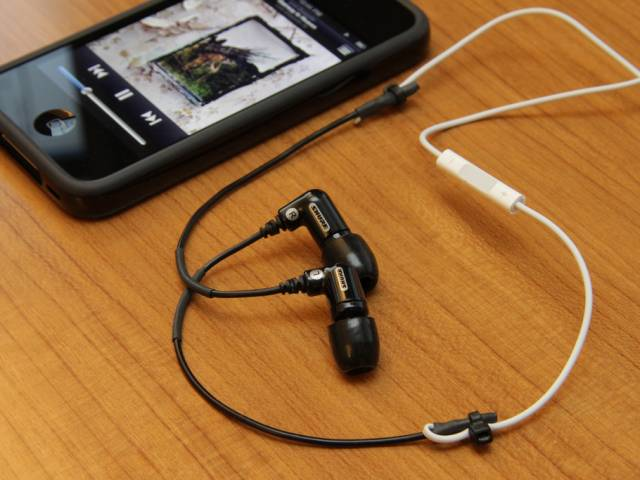
\includegraphics[width=\textwidth]{figures/dummy2.jpg}
\caption{Beispielbild mit Bildunterschrift unter dem Bild.}
\label{fig:grossesBild}
\end{figure}


\begin{figure}
\begin{captionbeside}[verkürzter Titel im Abbildungsverzeichnis]{Die Bildunterschrift kann bei schmaleren Abbildung auch seitlich an der Unterkante der Abbildung orientiert sein.}[3][\linewidth][.0\linewidth]*
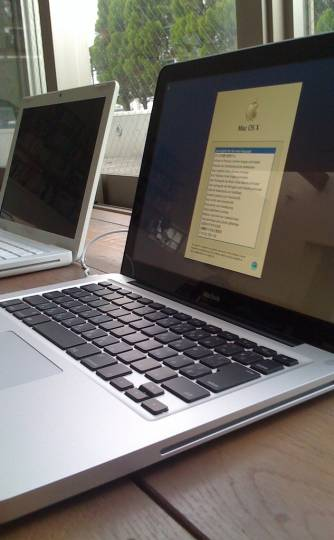
\includegraphics[width=0.4\textwidth]{figures/dummy1.jpg}
\end{captionbeside}
\label{fig:kleinesBild}
\end{figure}

\begin{table}[!h]   %[!htb]
\caption{Table in APA Format}
\small
\begin{tabular}{cccc}
\toprule
Column 1 & \multicolumn{3}{c}{Column 2} \\
\cmidrule(lr){2-4}
& Column 2a & Column 2b & Column2c \\
\midrule
a & 1 & .67 & 5 \\
b & 2 & .32 & 2 \\
c & 3 & .01 & 4 \\
\midrule
\multicolumn{4}{l}{\multirow{2}{90mm}{Note: This text is spanning 4 columns and 2 rows, and it is left justified.}} \\
\\
\bottomrule
\end{tabular}
\label{tab:apa-table}
\end{table}

\begin{table}[!h]%[!htb]
\caption{Monatsetat (in Euro)}
\begin{tabularx}{\textwidth}{@{}l*6{X}@{}}\toprule
        & N&        M&    s&     MD &    MIN &  MAX \\\midrule
Berufstätig &
       a          5 & 612 &    384 & 500 & 145\footnote{test} &   1017 \\
Nicht berufstätig & 21 & 485 & 272 & 436 & 0 &
              a                                      945 \\
Gesamt &      26 & 509 &    292 &     468 &    0&   1017 \\\midrule
\multicolumn{6}{@{}l}{{Note: text}} \\
\bottomrule
\end{tabularx}
\label{tab:monatsetat}
\end{table}

\section{Abbildungen und Tabellen}
Einführung einer \gls{abk} zum Beispiel: \Gls{http} mit Großbuchstaben am Anfang. Bei Zweitnennung wird nur die Kurzform dargestellt: \gls{http}. Das Abküzungsverzeichnis kann mit \texttt{\textbackslash printglossary[type=\textbackslash acronymtype]}  erzeugt werden.

%\section*{Main equations}
%\begin{equation}
%a=\frac{N}{A}
%\end{equation}%
%\nomenclature{$a$}{The number of angels per unit area}%
%\nomenclature{$N$}{The number of angels per needle point}%
%\nomenclature{$A$}{The area of the needle point}%
%The equation $\sigma = m a$%
%\nomenclature{$\sigma$}{The total mass of angels per unit area}%
%\nomenclature{$m$}{The mass of one angel}
%follows easily.
